% ============================================================
% ============================================================
% ============================================================
\section{Defining Classes in MATLAB}
% ============================================================
% ============================================================
% ============================================================

\subsection{The Class-definition File}
In MATLAB, we define a class using a class-definition file. The file name must be identical to the name of the class itself, and it must have the '\texttt{.m}' extension. For example, to define an \texttt{Asset} class, we create a file named '\texttt{Asset.m}' (without the single quotes, of course).

A class definition file may be obtained by the `\texttt{New Document}' button on the \texttt{Home} tab of the MATLAB IDE and selecting the `\texttt{Class}' option. This opens a new editor window with a textual template for your new class. An example of a new class template is shown in Fig. \ref{fig:EditorNewClass}. Alternately, one can simply select a new script and write the class from scratch.

Let us examine some of the features of the template class file generated for us by MATLAB 2017b (see Fig. \ref{fig:EditorNewClass}):
\begin{enumerate}
\item The class definition files begins the keyword \texttt{classdef}, followed immediately by the class name (line 1). Also, lines of comments immediately follow line 1, providing help documentation for the class. Together, the documentation comments and line 1 provide a class header. 
\begin{itemize}
\item In this case, the class template has the text \texttt{untitled5} as a placeholder for the class name.
\end{itemize}

\item Following the class header, there are two sections to the class definition:
\begin{itemize}
\item The \textbf{properties section} begins with the key word \texttt{properties} (line 5) and ends with the key word \texttt{end} (line 7).

The body of the \texttt{properties} section is used to define class properties (also known as ``fields'', or ``member data''). Here, there is one dummy property defined: \texttt{Property1}.

\item The \textbf{methods section} begins with the key word \texttt{methods} (line 9) and ends with the key word \texttt{end} (line 21).

The body of the \texttt{methods} section is used to define functions which operate on objects. Such functions are more precisely called \textbf{methods}.

\begin{itemize}
\item The first method is an important function known as a \textbf{constructor} method. The constructor function shares exactly the same name as the class, and is used to instantiate an object of the class. A constructor typically receives input arguments which are used to specify some object properties. Typically, a constructor has a single output, \texttt{obj}, which is the desired result of the constructor. Of all the class methods, the constructor is unique in the sense that it does not operate on nor is it associated with an existing object. All other method functions operate on at least one object, and thus require an object as the first input argument, typically \texttt{obj}.

In particular, the placeholder constructor method \texttt{untitled5()} sums input arguments \texttt{inputArg1} and \texttt{inputArg2} and stores the result in the lone object property \texttt{Property1}.

\item The second method, \texttt{method1()}, is of the typical, non-constructor form. The first input argument is an object, \texttt{obj}. %We say that the class method \texttt{method1()} is associated with the object \texttt{obj}.
Within a non-constructor method, the object \texttt{obj} is only a copy of the object passed to the function in the first argument. In particular, \texttt{method1()} sums \texttt{inputArg} and the object property \texttt{obj.Property1} and returns this result as \texttt{outputArg}. This function does not modify the original object. In fact, within \texttt{method1()}, the code actually works with a copy of the object specified by \texttt{obj}.%modifies the \textit{temporary} copy of \texttt{obj} by adding the second argument \texttt{inputArg} to the \texttt{Property1} property.
% The output is typically an object, and often the same object \texttt{obj} as in the first input. Under such circumstances, the modified copy of \texttt{obj} is returned to the invoking script or function when the execution of \texttt{method1()} concludes. The modified copy of \texttt{obj} within \texttt{method1()} is then used to overwrite the original version of \texttt{obj} in the invoking testbed function, thus modifying the object.
\end{itemize}

\end{itemize}

\end{enumerate}

% vvv------------------------------------------------------------vvv
\begin{figure}[htbp] %  figure placement: here, top, bottom, or page
   \centering
   \subfigure[ ]{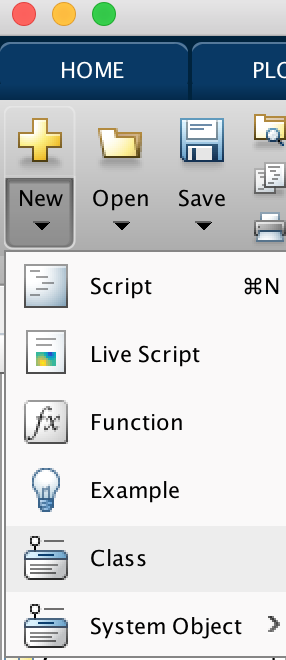
\includegraphics[height=2.5in]{graphics/NewDocumentClass.png}}
   \quad
   \subfigure[ ]{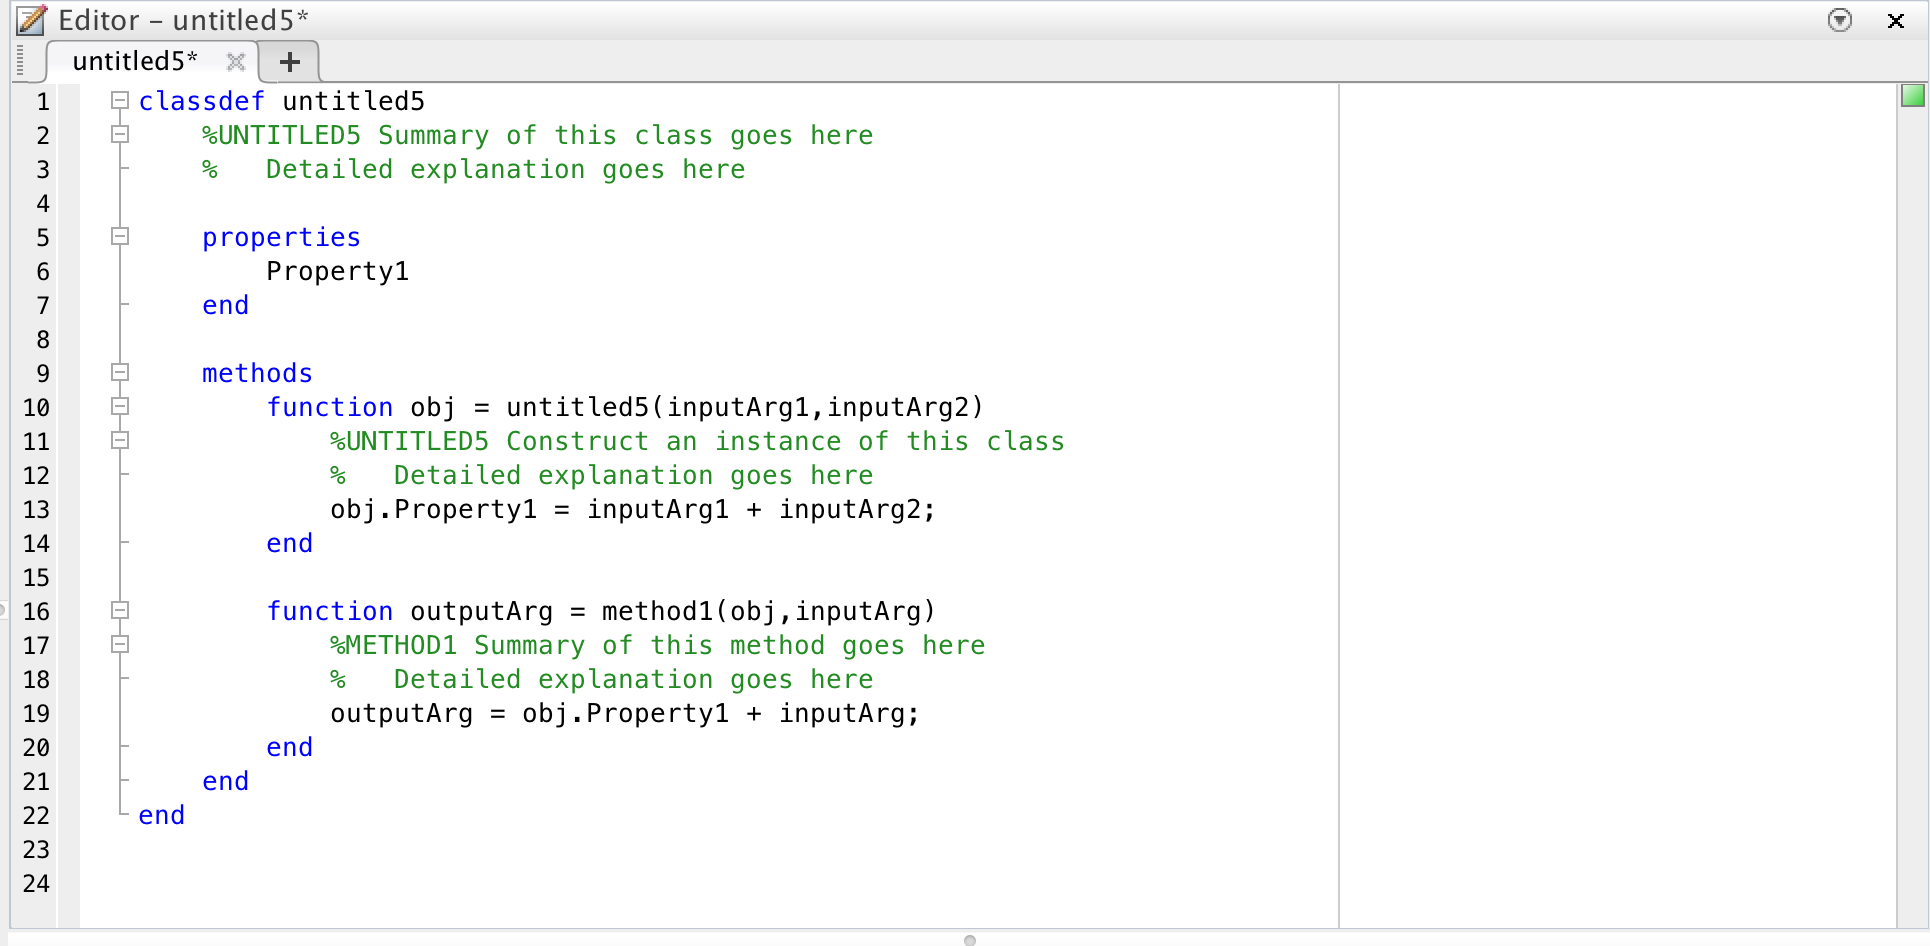
\includegraphics[height=2.5in]{graphics/MATLAB_Editor_NewClass.png}}
   \caption{(a) The ``New Document'' button provides a ``Class'' option. (b) A new class template obtained in MATLAB 2017b.}
   \label{fig:EditorNewClass}
\end{figure}
% ^^^------------------------------------------------------------^^^

\exmp{Example} \label{subsect:ConstructorUntitled5}
Create an object \texttt{myObj}.

\noindent \underline{Solution}.

To do this, we can invoke the constructor \texttt{untitled5()} using the syntax:
% vvv------------------------------------------------------------vvv
\begin{lstlisting}[style=Matlab-editor, caption={MATLAB Command Window input utilizing and testing the \texttt{untitled5} class definition of Fig.\ \ref{fig:EditorNewClass}.}]
>> x1 = 1; x2 = 2; myObj = untitled5(x1, x2)

myObj = 

  untitled5 with properties:

    Property1: 3
\end{lstlisting}
% ^^^------------------------------------------------------------^^^
Here, the command-line input of line 1 assigns the values 1 and 2 to \texttt{x1} and \texttt{x2}. Those values, then, are passed to the \texttt{untitled5()} constructor method to instantiate the object \texttt{myObj} of class \texttt{untitled5}. The output of this command is seen in lines 3-7, in which we see that \texttt{myObj} property \texttt{Property1} stores the value 3, which is the sum of the values stored in \texttt{x1} and \texttt{x2}.

\exmp{Invoke the method \texttt{method1()} on the object \texttt{myObj} created in Example \ref{subsect:ConstructorUntitled5}.}


\noindent \underline{Solution}.

To do this, invoke \texttt{method1()} using the syntax:
% vvv------------------------------------------------------------vvv
\begin{lstlisting}[style=Matlab-editor]
>> x = myObj.method1(5)

x =

     8
\end{lstlisting}
% ^^^------------------------------------------------------------^^^
To invoke \texttt{method1()} on \texttt{myObj}, we use the dot (``\texttt{.}'') syntax \texttt{myObj.method1(...)}, much like a reference to a property of \texttt{myObj}. This syntax is unique to class methods. While \texttt{myObj} does not appear within the input argument list to \texttt{method()} in line 1 above, it is in fact the first argument to \texttt{method()} because of the dot syntax. An alternative and equivalent\textemdash but older and depreciated\textemdash syntax for invoking \texttt{method1()} in line 1 above is \verb!x = method1(myObj, 5)!. This syntax explicitly specifies \texttt{myObj} as the first argument. The older syntax is used below, with the same result as above.
% vvv------------------------------------------------------------vvv
\begin{lstlisting}[style=Matlab-editor]
>> x = method1(myObj, 5)

x =

     8
\end{lstlisting}
% ^^^------------------------------------------------------------^^^

\subsubsection{Modifying Objects}
By default, when we pass an object to a method using either \texttt{obj.method1()} syntax or the older syntax, \textbf{only a copy of the object \texttt{obj} is passed to \texttt{method1()}}. Thus, any modifications \texttt{method1()} makes to its object are made to the \textit{copy}, not the original object.

If we wish to make a method \texttt{method2()} that modifies an object \texttt{myObj}, we need to define \texttt{method2()} in the following manner:
% vvv------------------------------------------------------------vvv
\begin{lstlisting}[style=Matlab-editor]
obj = method2(obj, InputArg1, InputArg2, ... )
      < statements that modify obj >
end
\end{lstlisting}
% ^^^------------------------------------------------------------^^^
Now, \texttt{method2()} returns the modified copy of the input object. The syntax to modify \texttt{myObj} is as follows:
% vvv------------------------------------------------------------vvv
\begin{lstlisting}[style=Matlab-editor]
myObj = myObj.method2( a, b, ... );
\end{lstlisting}
% ^^^------------------------------------------------------------^^^
This invocation of \texttt{method2()} allows \texttt{method2()} to modify a copy of \texttt{myObj}. Then, \texttt{method2()} returns a modified copy of \texttt{myObj}, which is used to overwrite the original, unmodified object \texttt{myObj}.

